\documentclass[tikz]{standalone}

\usepackage{pgfplots}
\pgfplotsset{compat=1.15}
\usepackage{mathrsfs}
\usetikzlibrary{arrows,calc}
\usepackage{tkz-euclide}
\pagestyle{empty}

\definecolor{AngleClr}{rgb}{0,0.39215686274509803,0}
\definecolor{ShapeClr}{rgb}{0.6,0.2,0}

\begin{document}

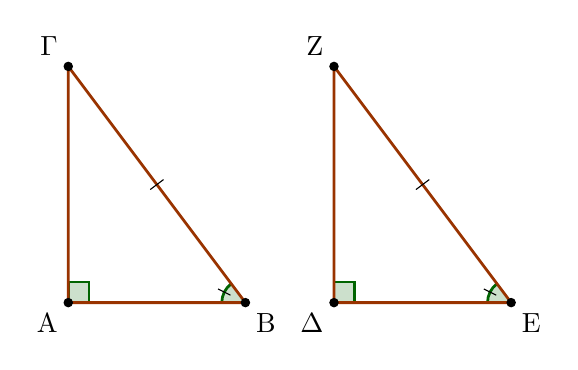
\begin{tikzpicture}[scale=.75]
\tkzSetUpLine[line width=1pt,color=black]
\tkzSetUpPoint[fill=black]

\tkzDefPoints{0/0/A,3/0/B,0/4/C}

\tkzDefPoints{4.5/0/D,7.5/0/E,4.5/4/Z}

\tkzFillPolygon[fill=white](A,B,C)
\tkzFillPolygon[fill=white](D,E,Z)


\tkzMarkRightAngles[line width=1pt, size=.35,color=AngleClr,fill=AngleClr,fill opacity=0.2](B,A,C E,D,Z)
\tkzFillAngles[fill=AngleClr,size=.4,fill opacity=0.2](C,B,A Z,E,D)
\tkzMarkAngles[mark=|,mksize=2.5,line width=1pt,size=.4,color=AngleClr](C,B,A Z,E,D)

\tkzDrawPolygons[color=ShapeClr](A,B,C D,E,Z)

\tkzDrawPoints[size=3](A,B,C,D,E,Z)

\tkzLabelPoint[below left](A){$\rm A$}
\tkzLabelPoint[below right](B){$\rm B$}
\tkzLabelPoint[above left](C){$\rm \Gamma$}

\tkzLabelPoint[below left](D){$\rm \Delta$}
\tkzLabelPoint[below right](E){$\rm E$}
\tkzLabelPoint[above left](Z){$\rm Z$}

\tkzMarkSegments[mark=|,size=3](B,C E,Z)

\end{tikzpicture}
\end{document}
